%==================================================================================================================
%============================================= Contexte ===========================================================
%==================================================================================================================

\section{Contexte}

\newsavebox{\cardbox}

\begin{frame}[t]{Contexte}
  \vspace{0.4em}
  % ---------- Première ligne : 420 ppm + double enjeu ----------------
  \savebox{\cardbox}{%
    \begin{minipage}{0.32\textwidth}
      \begin{pccard}
        \centering
        \vspace{0.3em}
        \pckeyfig{420~ppm}{Concentration actuelle de \ch{CO2} dans l'atmosphère}
        \vspace{0.3em}
      \end{pccard}
    \end{minipage}}
  \begin{columns}[T,onlytextwidth]
    \column{0.32\textwidth}
      \onslide<2->{\usebox{\cardbox}}
    \column{0.66\textwidth}
      \vspace*{-0.55cm}
      \onslide<1->{%
        \begin{pcbanner}{Un double enjeu : carbone et énergie}
          \begin{itemize}\footnotesize
            \item Demande énergétique mondiale croissante
            \item Carburants : seul stockage d'énergie à grande échelle
            \item Énergie solaire intermittente et difficile à stocker
            \item Valoriser le \ch{CO2} en molécules d'intérêt
                  $\rightarrow$ stockage de l'énergie solaire sous forme chimique
          \end{itemize}
        \end{pcbanner}}
  \end{columns}

  % ---------- Deuxième ligne : schéma (gauche, large) + GASPER -------
  \vspace{0.5em}
  \begin{columns}[T,onlytextwidth]
    \column{0.56\textwidth}
      \onslide<3->{%
        \begin{pcbanner}{Du \ch{CO2} aux carburants}
          \centering
          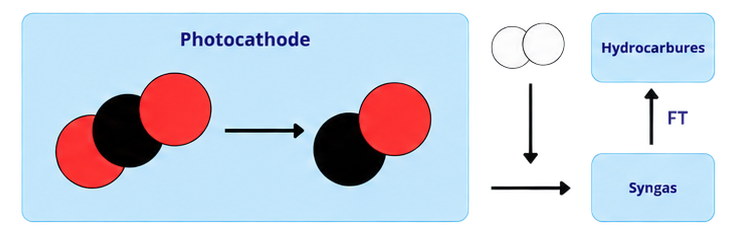
\includegraphics[width=0.98\linewidth]{schema_contexte.png}
        \end{pcbanner}}
    \column{0.42\textwidth}
      \onslide<4->{%
        \begin{pcbanner}{Projet ANR GASPER}
          \vspace{0.25em}
          \begin{itemize}\footnotesize
            \item Réduire le \ch{CO2} en \ch{CO} à l'aide d'une photocathode
            \item 6 laboratoires impliqués
            \item Élaboration, caractérisation et tests des photoélectrodes
            \item Objectifs : efficacité et sélectivité
          \end{itemize}
          \vspace{0.25em}
        \end{pcbanner}}
  \end{columns}
\end{frame}
%==================================================================================================================
%============================================= Fin Contexte =======================================================
%==================================================================================================================
